
%% bare_conf.tex
%% V1.4b
%% 2015/08/26
%% by Michael Shell
%% See:
%% http://www.michaelshell.org/
%% for current contact information.
%%
%% This is a skeleton file demonstrating the use of IEEEtran.cls
%% (requires IEEEtran.cls version 1.8b or later) with an IEEE
%% conference paper.
%%
%% Support sites:
%% http://www.michaelshell.org/tex/ieeetran/
%% http://www.ctan.org/pkg/ieeetran
%% and
%% http://www.ieee.org/

%%*************************************************************************
%% Legal Notice:
%% This code is offered as-is without any warranty either expressed or
%% implied; without even the implied warranty of MERCHANTABILITY or
%% FITNESS FOR A PARTICULAR PURPOSE!
%% User assumes all risk.
%% In no event shall the IEEE or any contributor to this code be liable for
%% any damages or losses, including, but not limited to, incidental,
%% consequential, or any other damages, resulting from the use or misuse
%% of any information contained here.
%%
%% All comments are the opinions of their respective authors and are not
%% necessarily endorsed by the IEEE.
%%
%% This work is distributed under the LaTeX Project Public License (LPPL)
%% ( http://www.latex-project.org/ ) version 1.3, and may be freely used,
%% distributed and modified. A copy of the LPPL, version 1.3, is included
%% in the base LaTeX documentation of all distributions of LaTeX released
%% 2003/12/01 or later.
%% Retain all contribution notices and credits.
%% ** Modified files should be clearly indicated as such, including  **
%% ** renaming them and changing author support contact information. **
%%*************************************************************************


% *** Authors should verify (and, if needed, correct) their LaTeX system  ***
% *** with the testflow diagnostic prior to trusting their LaTeX platform ***
% *** with production work. The IEEE's font choices and paper sizes can   ***
% *** trigger bugs that do not appear when using other class files.       ***                          ***
% The testflow support page is at:
% http://www.michaelshell.org/tex/testflow/



\documentclass[10pt, conference, compsocconf]{IEEEtran}
% Some Computer Society conferences also require the compsoc mode option,
% but others use the standard conference format.
%
% If IEEEtran.cls has not been installed into the LaTeX system files,
% manually specify the path to it like:
% \documentclass[conference]{../sty/IEEEtran}





% Some very useful LaTeX packages include:
% (uncomment the ones you want to load)


% *** MISC UTILITY PACKAGES ***
%
%\usepackage{ifpdf}
% Heiko Oberdiek's ifpdf.sty is very useful if you need conditional
% compilation based on whether the output is pdf or dvi.
% usage:
% \ifpdf
%   % pdf code
% \else
%   % dvi code
% \fi
% The latest version of ifpdf.sty can be obtained from:
% http://www.ctan.org/pkg/ifpdf
% Also, note that IEEEtran.cls V1.7 and later provides a builtin
% \ifCLASSINFOpdf conditional that works the same way.
% When switching from latex to pdflatex and vice-versa, the compiler may
% have to be run twice to clear warning/error messages.






% *** CITATION PACKAGES ***
%
%\usepackage{cite}
% cite.sty was written by Donald Arseneau
% V1.6 and later of IEEEtran pre-defines the format of the cite.sty package
% \cite{} output to follow that of the IEEE. Loading the cite package will
% result in citation numbers being automatically sorted and properly
% "compressed/ranged". e.g., [1], [9], [2], [7], [5], [6] without using
% cite.sty will become [1], [2], [5]--[7], [9] using cite.sty. cite.sty's
% \cite will automatically add leading space, if needed. Use cite.sty's
% noadjust option (cite.sty V3.8 and later) if you want to turn this off
% such as if a citation ever needs to be enclosed in parenthesis.
% cite.sty is already installed on most LaTeX systems. Be sure and use
% version 5.0 (2009-03-20) and later if using hyperref.sty.
% The latest version can be obtained at:
% http://www.ctan.org/pkg/cite
% The documentation is contained in the cite.sty file itself.






% *** GRAPHICS RELATED PACKAGES ***
%
\ifCLASSINFOpdf
  % \usepackage[pdftex]{graphicx}
  % declare the path(s) where your graphic files are
  % \graphicspath{{../pdf/}{../jpeg/}}
  % and their extensions so you won't have to specify these with
  % every instance of \includegraphics
  % \DeclareGraphicsExtensions{.pdf,.jpeg,.png}
\else
  % or other class option (dvipsone, dvipdf, if not using dvips). graphicx
  % will default to the driver specified in the system graphics.cfg if no
  % driver is specified.
  % \usepackage[dvips]{graphicx}
  % declare the path(s) where your graphic files are
  % \graphicspath{{../eps/}}
  % and their extensions so you won't have to specify these with
  % every instance of \includegraphics
  % \DeclareGraphicsExtensions{.eps}
\fi
% graphicx was written by David Carlisle and Sebastian Rahtz. It is
% required if you want graphics, photos, etc. graphicx.sty is already
% installed on most LaTeX systems. The latest version and documentation
% can be obtained at:
% http://www.ctan.org/pkg/graphicx
% Another good source of documentation is "Using Imported Graphics in
% LaTeX2e" by Keith Reckdahl which can be found at:
% http://www.ctan.org/pkg/epslatex
%
% latex, and pdflatex in dvi mode, support graphics in encapsulated
% postscript (.eps) format. pdflatex in pdf mode supports graphics
% in .pdf, .jpeg, .png and .mps (metapost) formats. Users should ensure
% that all non-photo figures use a vector format (.eps, .pdf, .mps) and
% not a bitmapped formats (.jpeg, .png). The IEEE frowns on bitmapped formats
% which can result in "jaggedy"/blurry rendering of lines and letters as
% well as large increases in file sizes.
%
% You can find documentation about the pdfTeX application at:
% http://www.tug.org/applications/pdftex



\usepackage{graphicx}

% *** MATH PACKAGES ***
%
%\usepackage{amsmath}
% A popular package from the American Mathematical Society that provides
% many useful and powerful commands for dealing with mathematics.
%
% Note that the amsmath package sets \interdisplaylinepenalty to 10000
% thus preventing page breaks from occurring within multiline equations. Use:
%\interdisplaylinepenalty=2500
% after loading amsmath to restore such page breaks as IEEEtran.cls normally
% does. amsmath.sty is already installed on most LaTeX systems. The latest
% version and documentation can be obtained at:
% http://www.ctan.org/pkg/amsmath





% *** SPECIALIZED LIST PACKAGES ***
%
%\usepackage{algorithmic}
% algorithmic.sty was written by Peter Williams and Rogerio Brito.
% This package provides an algorithmic environment fo describing algorithms.
% You can use the algorithmic environment in-text or within a figure
% environment to provide for a floating algorithm. Do NOT use the algorithm
% floating environment provided by algorithm.sty (by the same authors) or
% algorithm2e.sty (by Christophe Fiorio) as the IEEE does not use dedicated
% algorithm float types and packages that provide these will not provide
% correct IEEE style captions. The latest version and documentation of
% algorithmic.sty can be obtained at:
% http://www.ctan.org/pkg/algorithms
% Also of interest may be the (relatively newer and more customizable)
% algorithmicx.sty package by Szasz Janos:
% http://www.ctan.org/pkg/algorithmicx




% *** ALIGNMENT PACKAGES ***
%
%\usepackage{array}
% Frank Mittelbach's and David Carlisle's array.sty patches and improves
% the standard LaTeX2e array and tabular environments to provide better
% appearance and additional user controls. As the default LaTeX2e table
% generation code is lacking to the point of almost being broken with
% respect to the quality of the end results, all users are strongly
% advised to use an enhanced (at the very least that provided by array.sty)
% set of table tools. array.sty is already installed on most systems. The
% latest version and documentation can be obtained at:
% http://www.ctan.org/pkg/array


% IEEEtran contains the IEEEeqnarray family of commands that can be used to
% generate multiline equations as well as matrices, tables, etc., of high
% quality.




% *** SUBFIGURE PACKAGES ***
%\ifCLASSOPTIONcompsoc
%  \usepackage[caption=false,font=normalsize,labelfont=sf,textfont=sf]{subfig}
%\else
%  \usepackage[caption=false,font=footnotesize]{subfig}
%\fi
% subfig.sty, written by Steven Douglas Cochran, is the modern replacement
% for subfigure.sty, the latter of which is no longer maintained and is
% incompatible with some LaTeX packages including fixltx2e. However,
% subfig.sty requires and automatically loads Axel Sommerfeldt's caption.sty
% which will override IEEEtran.cls' handling of captions and this will result
% in non-IEEE style figure/table captions. To prevent this problem, be sure
% and invoke subfig.sty's "caption=false" package option (available since
% subfig.sty version 1.3, 2005/06/28) as this is will preserve IEEEtran.cls
% handling of captions.
% Note that the Computer Society format requires a larger sans serif font
% than the serif footnote size font used in traditional IEEE formatting
% and thus the need to invoke different subfig.sty package options depending
% on whether compsoc mode has been enabled.
%
% The latest version and documentation of subfig.sty can be obtained at:
% http://www.ctan.org/pkg/subfig




% *** FLOAT PACKAGES ***
%
%\usepackage{fixltx2e}
% fixltx2e, the successor to the earlier fix2col.sty, was written by
% Frank Mittelbach and David Carlisle. This package corrects a few problems
% in the LaTeX2e kernel, the most notable of which is that in current
% LaTeX2e releases, the ordering of single and double column floats is not
% guaranteed to be preserved. Thus, an unpatched LaTeX2e can allow a
% single column figure to be placed prior to an earlier double column
% figure.
% Be aware that LaTeX2e kernels dated 2015 and later have fixltx2e.sty's
% corrections already built into the system in which case a warning will
% be issued if an attempt is made to load fixltx2e.sty as it is no longer
% needed.
% The latest version and documentation can be found at:
% http://www.ctan.org/pkg/fixltx2e


%\usepackage{stfloats}
% stfloats.sty was written by Sigitas Tolusis. This package gives LaTeX2e
% the ability to do double column floats at the bottom of the page as well
% as the top. (e.g., "\begin{figure*}[!b]" is not normally possible in
% LaTeX2e). It also provides a command:
%\fnbelowfloat
% to enable the placement of footnotes below bottom floats (the standard
% LaTeX2e kernel puts them above bottom floats). This is an invasive package
% which rewrites many portions of the LaTeX2e float routines. It may not work
% with other packages that modify the LaTeX2e float routines. The latest
% version and documentation can be obtained at:
% http://www.ctan.org/pkg/stfloats
% Do not use the stfloats baselinefloat ability as the IEEE does not allow
% \baselineskip to stretch. Authors submitting work to the IEEE should note
% that the IEEE rarely uses double column equations and that authors should try
% to avoid such use. Do not be tempted to use the cuted.sty or midfloat.sty
% packages (also by Sigitas Tolusis) as the IEEE does not format its papers in
% such ways.
% Do not attempt to use stfloats with fixltx2e as they are incompatible.
% Instead, use Morten Hogholm'a dblfloatfix which combines the features
% of both fixltx2e and stfloats:
%
% \usepackage{dblfloatfix}
% The latest version can be found at:
% http://www.ctan.org/pkg/dblfloatfix




% *** PDF, URL AND HYPERLINK PACKAGES ***
%
%\usepackage{url}
% url.sty was written by Donald Arseneau. It provides better support for
% handling and breaking URLs. url.sty is already installed on most LaTeX
% systems. The latest version and documentation can be obtained at:
% http://www.ctan.org/pkg/url
% Basically, \url{my_url_here}.




% *** Do not adjust lengths that control margins, column widths, etc. ***
% *** Do not use packages that alter fonts (such as pslatex).         ***
% There should be no need to do such things with IEEEtran.cls V1.6 and later.
% (Unless specifically asked to do so by the journal or conference you plan
% to submit to, of course. )


% correct bad hyphenation here
\hyphenation{op-tical net-works semi-conduc-tor}


\usepackage{graphicx}
\usepackage{url}
\usepackage{amssymb}
\usepackage{color}
\usepackage{ifthen}


\usepackage{listings}


\setcounter{topnumber}{8}
\setcounter{bottomnumber}{8}
\setcounter{totalnumber}{8}
\renewcommand{\floatpagefraction}{.8}
\definecolor{mygreen}{rgb}{0,0.6,0}
\definecolor{mygray}{rgb}{0.5,0.5,0.5}
\definecolor{mymauve}{rgb}{0.58,0,0.82}

\definecolor{lightgray}{rgb}{.9,.9,.9}
\definecolor{darkgray}{rgb}{.4,.4,.4}
\definecolor{purple}{rgb}{0.65, 0.12, 0.82}
\lstdefinelanguage{JavaScript}{
	keywords={break, case, catch, continue, debugger, default, delete, do, else, false, finally, for, function, if, in, instanceof, new, null, return, switch, this, throw, true, try, typeof, var, void, while, with},
	deletekeywords={port},
	morecomment=[l]{//},
	morecomment=[s]{/*}{*/},
	morestring=[b]',
	morestring=[b]",
	ndkeywords={class, export, boolean, throw, implements, import, this},
	keywordstyle=\color{blue}\bfseries,
	ndkeywordstyle=\color{darkgray}\bfseries,
	identifierstyle=\color{black},
	commentstyle=\color{purple}\ttfamily,
	stringstyle=\color{red}\ttfamily,
	sensitive=true
}

\lstset{
	language=JavaScript,
		deletekeywords={port},
	backgroundcolor=\color{lightgray},
	extendedchars=true,
	basicstyle=\footnotesize\ttfamily,
	showstringspaces=false,
	showspaces=false,
	numbers=left,
	numberstyle=\footnotesize,
	numbersep=9pt,
	tabsize=2,
	breaklines=true,
	showtabs=false,
	captionpos=b
}
\lstdefinelanguage{ThingML}{%
	language     = C,
	morekeywords = {action,port,required,end,statechart,state,on,entry,action,sends,function},
	otherkeywords={action,statechart,init,entry,stream, from,select,filter,thing,message,includes,provided,receives,function,internal,action,guard,event,port,function,var},           % 
}

\lstset{ %
	backgroundcolor=\color{white},   % choose the background color; you must add \usepackage{color} or \usepackage{xcolor}
	basicstyle=\footnotesize,        % the size of the fonts that are used for the code
	breakatwhitespace=false,         % sets if automatic breaks should only happen at whitespace
	breaklines=true,                 % sets automatic line breaking
	captionpos=b,                    % sets the caption-position to bottom
	commentstyle=\color{mygreen},    % comment style
	%	deletekeywords={},            % if you want to delete keywords from the given language
	escapeinside={\%*}{*)},          % if you want to add LaTeX within your code
	extendedchars=true,              % lets you use non-ASCII characters; for 8-bits encodings only, does not work with UTF-8
	frame=single,	                   % adds a frame around the code
	keepspaces=true,                 % keeps spaces in text, useful for keeping indentation of code (possibly needs columns=flexible)
	keywordstyle=\color{blue},       % keyword style
	language=ThingML,                 % the language of the code
	otherkeywords={stream, from,select,filter,thing,message,init,includes,provided,sends,receives,function,internal,action,guard,event},           % if you want to add more keywords to the set
	numbers=left,                    % where to put the line-numbers; possible values are (none, left, right)
	numbersep=5pt,                   % how far the line-numbers are from the code
	numberstyle=\tiny\color{mygray}, % the style that is used for the line-numbers
	rulecolor=\color{black},         % if not set, the frame-color may be changed on line-breaks within not-black text (e.g. comments (green here))
	showspaces=false,                % show spaces everywhere adding particular underscores; it overrides 'showstringspaces'
	showstringspaces=false,          % underline spaces within strings only
	showtabs=false,                  % show tabs within strings adding particular underscores
	stepnumber=2,                    % the step between two line-numbers. If it's 1, each line will be numbered
	stringstyle=\color{mymauve},     % string literal style
	tabsize=2,	                   % sets default tabsize to 2 spaces
	title=\lstname                   % show the filename of files included with \lstinputlisting; also try caption instead of title
}


% One command per author:
\newboolean{showcomments}
\setboolean{showcomments}{true}
%\setboolean{showcomments}{false}
\ifthenelse{\boolean{showcomments}}
 { \newcommand{\mynote}[2]{
      \fbox{\bfseries\sffamily\scriptsize#1}
        {\small$\blacktriangleright$\textsf{\textcolor{red}{{\em #2}\bf }}$\blacktriangleleft$}}}
        { \newcommand{\mynote}[2]{}}
%\newcommand{\ff}[1]{\mynote{Francois}{#1}}
%\newcommand{\mt}[1]{\mynote{Max}{#1}}
\newcommand{\ff}[1]{}
\newcommand{\mt}[1]{}


\begin{document}
%
% paper title
% Titles are generally capitalized except for words such as a, an, and, as,
% at, but, by, for, in, nor, of, on, or, the, to and up, which are usually
% not capitalized unless they are the first or last word of the title.
% Linebreaks \\ can be used within to get better formatting as desired.
% Do not put math or special symbols in the title.
\title{KevoreeJS: Enabling dynamic software reconfigurations in the Browser}


% author names and affiliations
% use a multiple column layout for up to three different
% affiliations
\author{\IEEEauthorblockN{Maxime Tricoire, Olivier Barais,\\ Manuel Leduc, Johann Bourcier}
\IEEEauthorblockA{INRIA, IRISA, Universit\'e de Rennes 1\\
Rennes, France\\
firstname.name@irisa.fr}
\and
\IEEEauthorblockN{Fran\c cois Fouquet,\\ Gr\'egory Nain, Ludovic Mouline}
\IEEEauthorblockA{SnT, Luxembourg\\
firstname.name@uni.lu}
\and
\IEEEauthorblockN{Gerson Sunye}
\IEEEauthorblockA{INRIA, Universit\'e de Nantes\\
gerson.sunye@inria.fr}

\and
\and
\IEEEauthorblockN{Brice Morin}
\IEEEauthorblockA{Sintef\\
Oslo, Norway\\
bmorin@sintef.no}}

% conference papers do not typically use \thanks and this command
% is locked out in conference mode. If really needed, such as for
% the acknowledgment of grants, issue a \IEEEoverridecommandlockouts
% after \documentclass

% for over three affiliations, or if they all won't fit within the width
% of the page, use this alternative format:
%
%\author{\IEEEauthorblockN{Michael Shell\IEEEauthorrefmark{1},
%Homer Simpson\IEEEauthorrefmark{2},
%James Kirk\IEEEauthorrefmark{3},
%Montgomery Scott\IEEEauthorrefmark{3} and
%Eldon Tyrell\IEEEauthorrefmark{4}}
%\IEEEauthorblockA{\IEEEauthorrefmark{1}School of Electrical and Computer Engineering\\
%Georgia Institute of Technology,
%Atlanta, Georgia 30332--0250\\ Email: see http://www.michaelshell.org/contact.html}
%\IEEEauthorblockA{\IEEEauthorrefmark{2}Twentieth Century Fox, Springfield, USA\\
%Email: homer@thesimpsons.com}
%\IEEEauthorblockA{\IEEEauthorrefmark{3}Starfleet Academy, San Francisco, California 96678-2391\\
%Telephone: (800) 555--1212, Fax: (888) 555--1212}
%\IEEEauthorblockA{\IEEEauthorrefmark{4}Tyrell Inc., 123 Replicant Street, Los Angeles, California 90210--4321}}




% use for special paper notices
%\IEEEspecialpapernotice{(Invited Paper)}


% make the title area
\maketitle

% As a general rule, do not put math, special symbols or citations
% in the abstract
\begin{abstract}

\ff{I would claim something stronger, about the mobility and inescable move to mobile app used on modile, web and so} 
The architecture of classic productivity software are moving from a traditional desktop-based software to a client server architecture hosted in the Cloud.    
In this context, web browsers behave as application containers that allow users to access a variety of Cloud-based applications and services, such as IDEs, Word processors, Music Collection Managers, etc.
As a result, a significant part of these software run in the browser and accesses remote services.
\ff{maybe for the CBSE community we could use another example than rich application, we can for instance use one really from backend oriented technology in order to make clear that we want to port it to web}
A lesson learned from development framework used in distributed applications is the success of pluggable architecture pattern as a core architecture concept,  i.e.,  a Software Architecture that promotes the use of Pluggable Module to dynamically plug. 
Following this trend, this paper discusses the main challenges to create a component-based platform supporting the development of dynamically adaptable single web page applications.
This paper also presents an approach called KevoreeJS based on models@runtime to control browser as component platform which address some of these challenges.
We validate this work by presenting the design of a dashboard for sensor based system and highlighting the capacity of KevoreeJS to dynamically choose the placement of code on the server or client side and how KevoreeJS can be used to dynamically install or remove running components.
\ff{buzz sentence to include like: driving browser as component platform?}


\end{abstract}

\smallskip
\noindent \textbf{Keywords.} \textit{Web Engineering, Dynamic component model, 	Single page application}.


% no keywords




% For peer review papers, you can put extra information on the cover
% page as needed:
% \ifCLASSOPTIONpeerreview
% \begin{center} \bfseries EDICS Category: 3-BBND \end{center}
% \fi
%
% For peerreview papers, this IEEEtran command inserts a page break and
% creates the second title. It will be ignored for other modes.
\IEEEpeerreviewmaketitle


\section{Introduction}

Traditional desktop-based productivity software moves to the Cloud. 
Nowadays, the browser is essentially an application container that allows users to run a single page application to  access a variety of Cloud-based applications and services that can be IDE, Word processor, Music Collection Manager, etc. 
A large offer of generative framework now propose to create the skeleton of such modern web applications, such as cite JHipster\footnote{https://jhipster.github.io/}, Mean.js~\footnote{http://meanjs.org}, ionic\footnote{http://ionicframework.com/}, keystonejs\footnote{http://keystonejs.com/}... 
These stacks generally use frameworks for developing the client part following a family of MVC pattern such as AngularJS~\cite{green2013angularjs}, emberjs~\cite{cravens2014building}, backbone~\cite{osmani2013developing}, durandal~\cite{monteiro2014learning}, react~\cite{fedosejev2015react}.  

\ff{same remarks than abstract i would use another exemple to motivate the use of CBSE techniques}
A lesson learnt from classical rich application development framework used for building IDE, word processor, music or video player is the success of the use of the pluggable or composite architecture pattern~\cite{115158,schmidt2013pattern} as a core architecture concept,  i.e. a Software Architecture that allows dynamically plugging functionality using Pluggable Modules to tune its applications to its project requirements. In this trend, the OSGi framework specification~\cite{hall2011osgi} has been widely adopted by the Eclipse community and forms the basis of the Eclipse Runtime since Eclipse 3.X. The OSGi framework is a module system and service platform for the Java programming language that implements a complete and dynamic component model. Components (coming in the form of bundles for deployment) can be remotely installed, started, stopped, updated, and uninstalled without requiring a reboot.  

The design of highly configurable web applications requires the support of such pluggable architecture based on Component Based Software Engineering within the Browser. Current framework such as AngularJS, ember, backbone, durandal or react focus on a clear architecture of the web applications following a single page application principle~\cite{monteiro2014learning} but does not provide a solution to dynamically reconfigure a running application. Due to the increasing complexity of Web Applications and based on the experience of other applications container, it is now required to support the evolution of a software artefact or the installation of a new software artefact without reloading the web page.  

This paper mainly highlights the challenges that arise when supporting a pluggable architecture pattern that enables the dynamic reconfiguration of a single page application. It also presents KevoreeJS in details, our approach to provide such a platform, and discuss its current limitations. We validate this work by showing how KevoreeJS can help to dynamically change Client/Server code partitioning in a dashboard for sensor-based system. Through this use case, we motivate the need for a dynamic module system for the browser, similar to OSGi for the JVM.  

The remainder of this paper is the following. Section 2 presents the main challenges for designing a module system for the JavaScript programming language that implements a complete and dynamic component model. Section 3 shows an overview of KevoreeJS and illustrates the main concepts through a motivating example of a dashboard for sensor based systems. Section 4 and 5 discuss related work and present ongoing work. 
\section{Main challenges for the use of the browser as a container for reconfigurable single page web applications }
A single-page application (SPA) is a web application that fits on a single web page, providing a more fluent user experience similar to a desktop application.
This architecture style is now a standard way of designing modern Web applications, but still lacks support for dynamic reconfigurability.
\ff{SPA has impact on browser caching, and enforce more easilly a dynamic web page construction based on data. Maybe we should extends a bit here to make this clear}
This section discusses eight important challenges to  enable dynamic reconfigurability in a SPA.

\subsection{Automatically provision component implementation and third-party libraries}

Component-based distributed systems are known to be hard to deploy for two main reasons: the complexity of their structure and the complexity of the deployment tasks. Most of the current tools are not able to properly address these challenges because the component dependency descriptions they rely on lack expressiveness. Web modules does not avoid this drawback. Indeed if most of them use tools to manage dependencies at design time such as node package manager (npm\footnote{https://www.npmjs.com/}) or bower\footnote{http://bower.io/}, this tools are  generally not used to enable the dynamic loading of third parties library at runtime. Besides, deploying component in the web is generally done when the user access the web page. In Web applications, updates are made by downloading new software artefacts when the user refresh the whole page. In a SPA, either all necessary code -- HTML, JavaScript, and CSS -- is retrieved with a single page load, usually in response to user actions. The page does not reload at any point in the process, nor does control transfer to another page, although the location hash can be used to provide the perception and navigability of separate logical pages in the application. SPA Frameworks provide solutions to  avoid waiting for pages to load and to support dynamic updates of page fragments. However, this mechanism never includes the integration of the update of existing libraries. The first challenge for building dynamically adaptable single page web applications is to manage the dynamic deployment of new components and their third-parties libraries without perturbing the running applications. It includes also a correct management of libraries dependencies based on standard tooling used by developers such as bower or npm.

\ff{maybe an idea to extend here would be to speak about CDNJS, and similar approach where they try to provision SPA without only the use of server. This approach is pretty similar to this idea of CBSE driven provisioning. Either we put a remark here and wait for the contribution, either we just introduce CDNJS}

\subsection{Type System}
The second main challenge is to make web components contract-aware~\cite{beugnard1999making}. If the CBSE community agrees to trust a component, we must be able to determine how this component will behave. The Web domain is far from the development method used for  mission-critical applications. Web developers generally use JavaScript as a programming language without providing a clear interface for their components. A component model for Web Application must force the developer to declare component interface and propose at minimum a basic level of contract to support duck typing verification when assembling components~\cite{beugnard1999making}. These contracts can also be used to check that the component interface fully conforms to its implementation if developers used  programming language such as TypeScript~\cite{rastogi2015safe} or Dart~\cite{dhiman2012google} to implement its components.
\ff{this could sounds like an attack point, if WebDev don't care about type, why they will use a modularized systems? :-) We should just turn and reverse the sentence to make this obviouss}

\subsection{User Interface composition}
The next challenge is to provide a way to compose the User Interface (UI). If HTML-based interface technologies enable end-users to easily use various remote Web applications, it is difficult for end-users to express complex compositions. Currently, the main Web actors provide framework to express complex compositions, such as react~\cite{fedosejev2015react} from Facebook that provides an adaptation algorithm to compute the minimum diff in the DOM. Google's polymer~\footnote{https://www.polymer-project.org/1.0/} is a similar approach with stronger emphasis on reusability. RiotJS~\footnote{http://riotjs.com/} also provides a lightweight framework for UI composition, however limited to static composition.
None of them are aims at providing dynamically reconfigurable user interface composition mechanism for the deployed components.
%\ff{The last sentence is an attack point :-), should be protected}

\subsection{Security handling}
Providing reconfigurations support from an external manager leads to several security issues.
If the SPA can receive a new configuration, automatically download components and update the running ones, it becomes easy to disseminate malware to any running application.
The model which is the blueprint of the deployed runtime system should embed mechanisms to ensure authentication and the data integrity of the system.
\ff{it is not that this is not new, the claim is more that remote CBSE will not introdcuce new problems and therefore can rely on existing already deployed protecting solutions, such as HTTPS}
This kind of issue is not new to the world of web development and existing principles can be applied such as https protocols, Role-based access control\dots

\subsection{Search engine optimization}
Because of the lack of JavaScript execution on crawlers of some popular Web search engines, SEO (Search engine optimization) has historically presented a problem for public facing websites wishing to adopt the SPA model. In fact modern Web search engine such as google support the fact that a SPA can dynamically generate new contents~\cite{googlesearch}. However, in the case of a dynamic component model, the crawler cannot know in advance all the components that can be installed in a web application. Consequently, search engines that only know the first configuration of the application cannot correctly index such a dynamically reconfigurable SPA. This require to integrate new metadata to define, for example, all the components that can be installed on a running web app. In that case, a search engine can do the hypothesis of the closed world to know all the potential configurations of a Web application (even if it can become combinatorial).
\ff{Definitevely true and a very interesing point. However, maybe we should turn it a little bit more positive. Like saying what could be open taks to pave the way towards a tighter integration of crawler and dynamic SPA (if we have to call them)}

\subsection{Client/Server code partitioning}
A dynamic component model for SPA must enable dynamic client/server code partitioning. In that sense such framework must provide abstractions for templating definition and rendering, abstraction for streams queries, … to let a developer change dynamically if the component is executed within the browser or at the server side. As it exists lots of technical stack at the server side that uses different programming languages, the component model must provide abstractions to define the component behavior that can be generated to this different technical stacks. In some simple case, we could imagine to do the hypothesis that the server also used JavaScript. In that case, it exists initial solutions \footnote{http://isomorphic.net/ references a set of solutions for client/server partitioning} to let share the same code for the client and the server side.

\subsection{Browser history}
With an SPA being, by definition, "a single page", the model breaks the browser's design for page history navigation using the Forward/Back buttons. The traditional solution for SPAs has been to change the browser URL's hash fragment identifier in accord with the current screen state.
The HTML5 specification has introduced \textit{pushState} and \textit{replaceState} providing programmatic access to the actual URL and browser history.
For a dynamic component model, the main challenge is to defined how to aggregate the states of the many deployed components.
The second challenge is to specify if a user request to go back to a previous state, does it include to come back to a previous configuration?
There is in fact several histories in a dynamically reconfigurable SPA: history of actions, history for caching of data, etc.



\subsection{Analytics}

Analytics is a common concerns for web applications. The goal is to be able to track and report website traffic and user activity.
%\ff{Analytics is very wide :-) what kind of analytic is part of the challenge here :)?s}
Tools such as Google Analytics rely heavily upon entire new pages loading in the browser, initiated by a URL change. As SPAs do not work this way, and in particular if we dynamically load new components analytics package has no idea who is doing what on the web applications.
The new HTML5 history API allows to add page load events to an SPA.
As the component web developers is in charge of using correctly this API, the challenge is then to avoid missing reports and double entries   .

Analytics, browser history and Search engine optimization are clearly challenging due to dynamics requirements.

\subsection{Speed of initial load (overhead @ runtime) }
The last challenge is to guarantee the flexibility offered by the use of a pluggable architecture does not introduce too much overhead when we start the SPA. Such an approach must guarantee to  avoid excessive downloading of unused features.

\ff{The first load is just the observable part, however the real overhead is server rendering versus browser rendering, i.e. asembly of GUI pieces...}

\section{KevoreeJS: A runtime for reconfigurable single page applications in the browser}

This section present a module system for the Browser called KevoreeJS . 
%\ff{Just matter of presention, but i think we not target JS, we target the brower USING javascript. But the goal is really to target a usage and not a language no ? The language is a way todo.}
In particular, KevoreeJS implements a dynamic component model for SPA. 
This component model currently addresses only a part of the challenges discusses in Section 2.   

\subsection{Motivating Scenarios }
To illustrate the framework, we consider a simple dashboard for sensor-based system in which, it is required to install/uninstall a new web widget when a new sensor appears/disappears. In such system, three kinds of reconfiguration has to be managed: i) the installation and retrieval of software package (javascript code), the instantiation of components, the components parametrization (to bind components through ports, the setup of parameters, ...), the component life-cycle management. ii)  the client/server code partitioning to select if some components that manage complex event queries must be executed on the server side or within the browser. iii) the selection of a specific  deploy unit depending on the browser type, its devices and its screen layout. A figure of the results of such an application is presented in Figure\ref{fig:fig1}.   This dashboard provides information regarding values that can come from a set of nodes such as the one described in Figure~\ref{fig:fig2}


\begin{figure}[h]
	\centering
	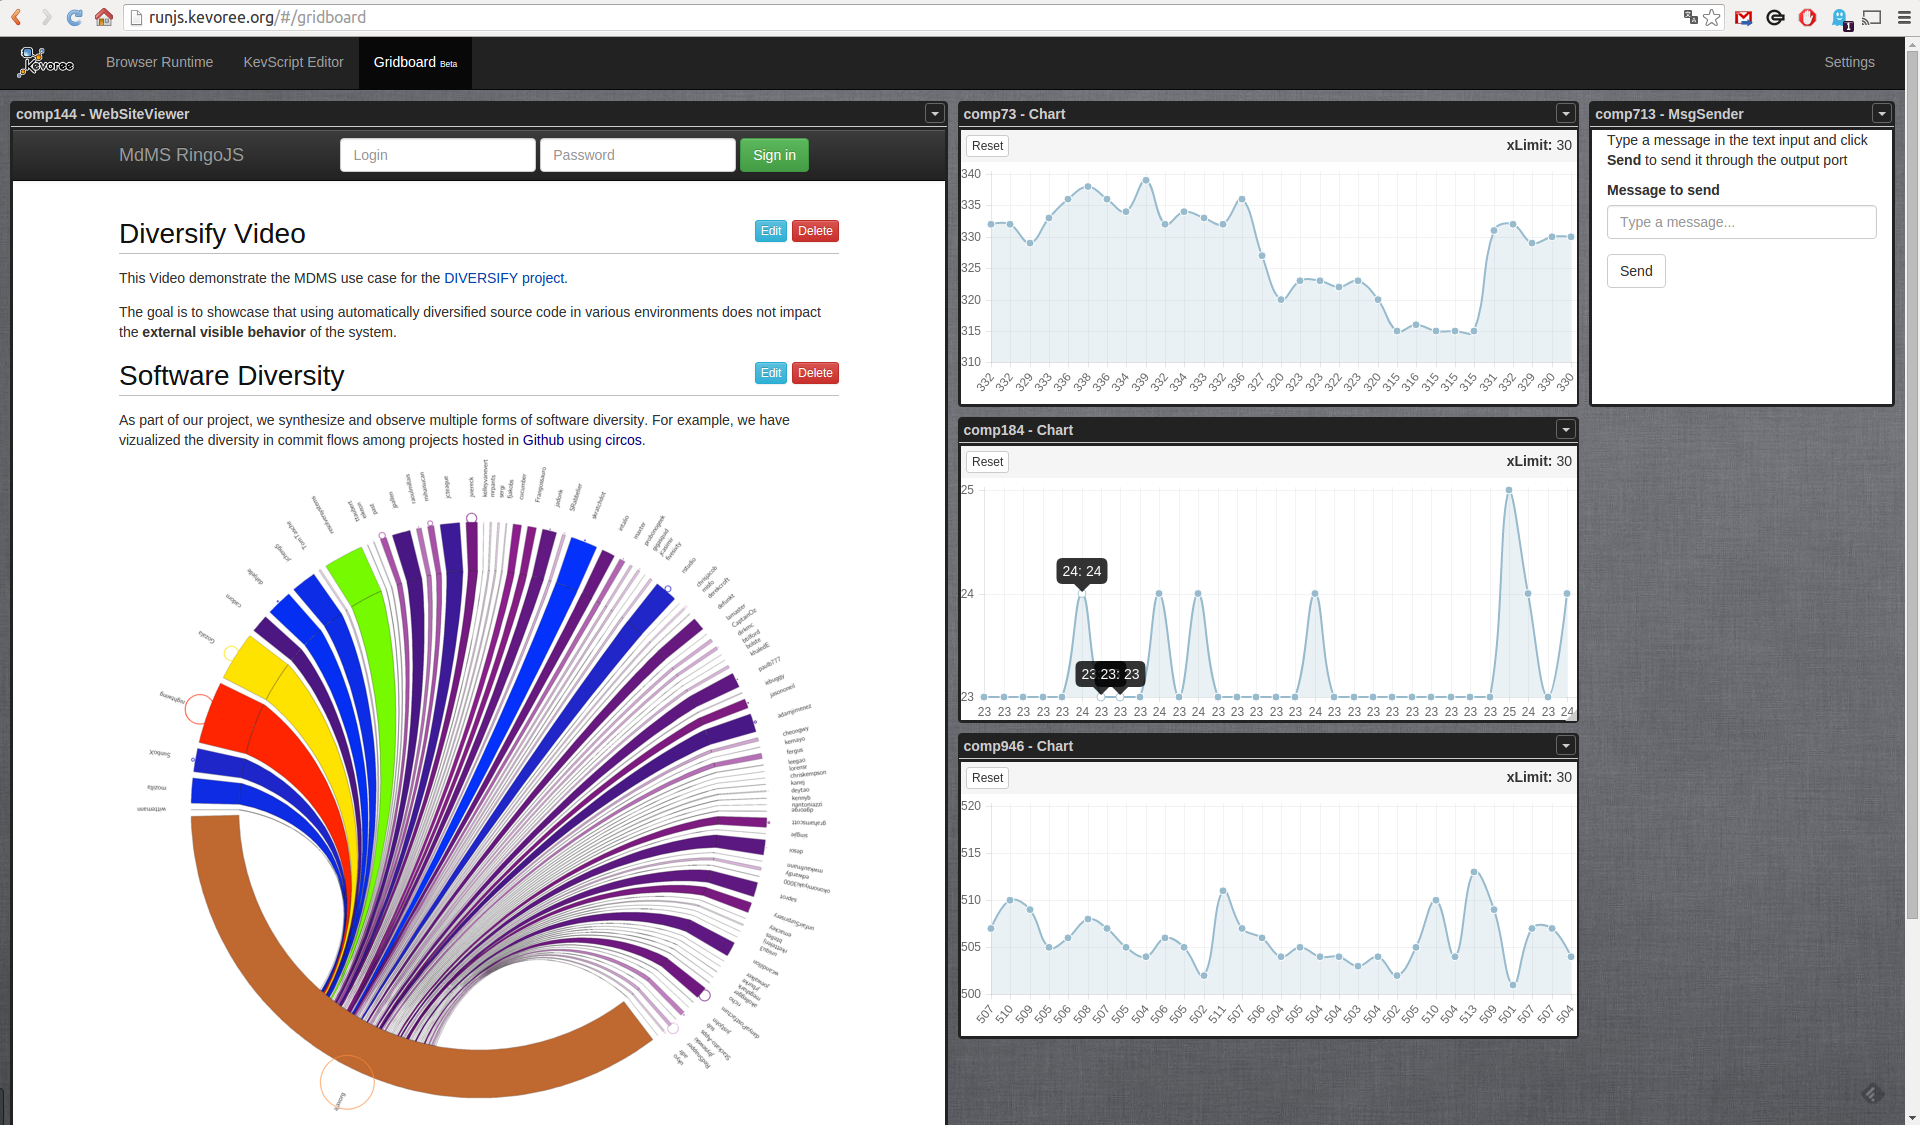
\includegraphics[width=1\linewidth]{figures/fig3}
	\caption{An example of dashboard for sensor-based applications}
	\label{fig:fig1}
\end{figure}


\begin{figure}[h]
	\centering
	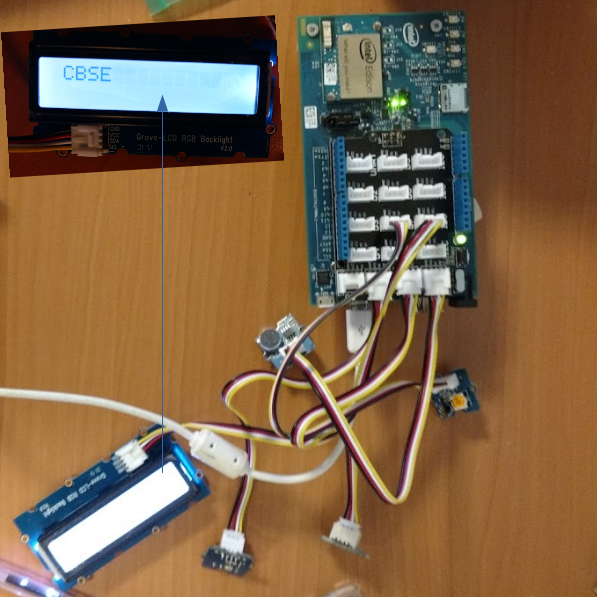
\includegraphics[width=0.8\linewidth]{figures/fig4}
	\caption{An example of sensor node based on Intel Edison}
	\label{fig:fig2}
\end{figure}


\subsection{KevoreeJS overview }
KevoreeJS is built on top of models@runtime paradigm. Models@runtime denotes model-driven approaches aiming at taming the complexity of dynamic adaptation. It basically pushes the idea of reflection~\cite{DBLP:conf/icse/MorinBNJ09} one step further by considering the reflection layer as a real model that can be used to drive the system deployment and (re) configuration: ``something simpler, safer or cheaper than reality to avoid the complexity, danger and irreversibility of reality''. In practice, component-based (and/or service-based) platforms like Fractal~\cite{bruneton2006fractal}, OpenCOM~\cite{grace2005reflective} or OSGi~\cite{hall2011osgi} offer reflection APIs which make it possible to introspect the system (which components and bindings are currently in place in the system) and dynamic adaptation (by applying CRUD operations on these components and bindings). While some of these platforms offer rollback mechanisms~\cite{david2006safe} to recover after an erroneous adaptation, the idea of models@runtime is to prevent the system from actually enacting an erroneous adaptation. In other words, the ``model at runtime'' is a reflection model which can be uncoupled (for reasoning, validation, simulation purposes) and automatically resynchronized. This modelling layer provides a common abstraction to describe the system configuration. this model can be interpreted to decide which packages (component package and third parties libraries) must be installed or removed and which component must be instantiated and started. This modelling layer can be also modified and push to peers to trigger distributed reconfigurations. 

KevoreeJS\footnote{http://runjs.kevoree.org}  implements the Kevoree component model. Kevoree is a dynamic component-based framework for distributed systems that follows the models@runtime paradigm and embeds a structural model of the distributed system. This model is used for two main purposes: (i) it represents a snapshot of the heterogeneous and distributed application state and (ii) it provides a language to drive the reconfiguration of this application. The Kevoree model embodies the following four main concepts of a distributed system. 

\begin{enumerate}
	\item The software \textbf{components} represent software units that provide the business value of the distributed system. 
\item The \textbf{connectors} (called channels in Kevoree) are in charge of inter-component communication. A channel encapsulates and provides a particular communication semantic (e.g. synchronous or asynchronous, unicast or multicast, and may provide different contracts for synchronization and quality of services). 
\item The \textbf{nodes} represent execution hosts for all other software entities such as components and channels. A node may represent a physical node or a virtual machine. Nodes are application containers and they are in charge of the dynamic adaptation of its system part when a new model@runtime is received. 
\item The \textbf{groups} are responsible for inter-node communication. In particular, a group provides semantics of dissemination and ensures consistency of models among nodes. On top of these abstractions, Kevoree provides a development model to design new components, channels, groups and containers using different programming languages. It also comes with a set of tools for building dynamic applications (a graphical editor to visualize and edit configurations, a textual language to express reconfigurations, several checkers to validate configurations). Kevoree supports multiple execution platforms (e.g., Java, Android, LXC, Docker, FreeBSD, Arduino). For each target platform it provides a specific runtime container as a specific node type. 

\end{enumerate}


For supporting the SPA within the browser, we mainly reuse the core of Kevoree component model which is written in Kotlin. This core contains the component model entities, tooling for loading and saving configuration models, tooling for detecting abstract actions (install a library, instantiate a component, bind a component to a channel, …)  and tooling to achieve runtime adaptations when the platforms receive a new configuration model. As Kotlin provides code generators for JavaScript, we can reuse this core tool directly. As a consequence, to create KevoreeJS we mainly provide the concrete implementations of abstract actions in order to achieve concrete tasks within a running Browser core. We also provide a basic UI composition mechanism based on mashup. Each component comes with its own view that can be composed on the full SPA using mashup. To enable this mashup mechanism, we reuse framework such as AngularJS and angular-gridster. KevoreeJS reuses bower for its static Web part, but it handles the dynamicity by downloading browserified\footnote{http://browserify.org/} modules directly from the npm registry. 


Finally we provide a simple development model in JavaScript and in TypeScript for developing component, channel or  group. This development model are available online\footnote{ https://github.com/HEADS-project/training/tree/master/2.Kevoree\_Basics}, \footnote{https://github.com/kevoree/kevoree-js.d.ts }.  

KevoreeJS comes with a set of tools: a web-based architecture model editor, a Yeoman generator, a set of Grunt tasks to fully automate the component packaging and publishing and a container to manage the dynamic deployment of third-party libraries. 

\subsection{Evaluation} 
To validate the proposed approach, we mainly follow two ways. First we provide some figures on KevoreeJS in terms of line of code, number of reusable component available online, time penalty to load initiate KevoreeJS when loading the pages. Next, we evaluate the approach regarding the challenges discussed in Section 2. 

\subsubsection{Quantitative evaluation}
To implement the KevoreeJS core and the sensor based dashboard, we create 8 components, 3 channels, 3 groups. The core of KevoreeJS and these 14 software artefacts contain 56,671 LoC (15,584 has been manually written and 41,177 are generated from the model to automatically manage model entities, model load and serialization, \dots The Figure~\ref{fig:fig3}  illustrates the configuration model of the applications using the Kevoree Web Editor~\footnote{http://editor.kevoree.org}. The Figure \ref{fig:fig4} focuses in particular on the configuration of the SPA presented in Figure~\ref{fig:fig1}. All the code for this application is available on github. We provide a companion web page \footnote{http://github.com/kevoree/CBSE16KevoreeJS} to provide the links to all the software artefacts we use in this experiment.  


\begin{figure}[h]
	\centering
	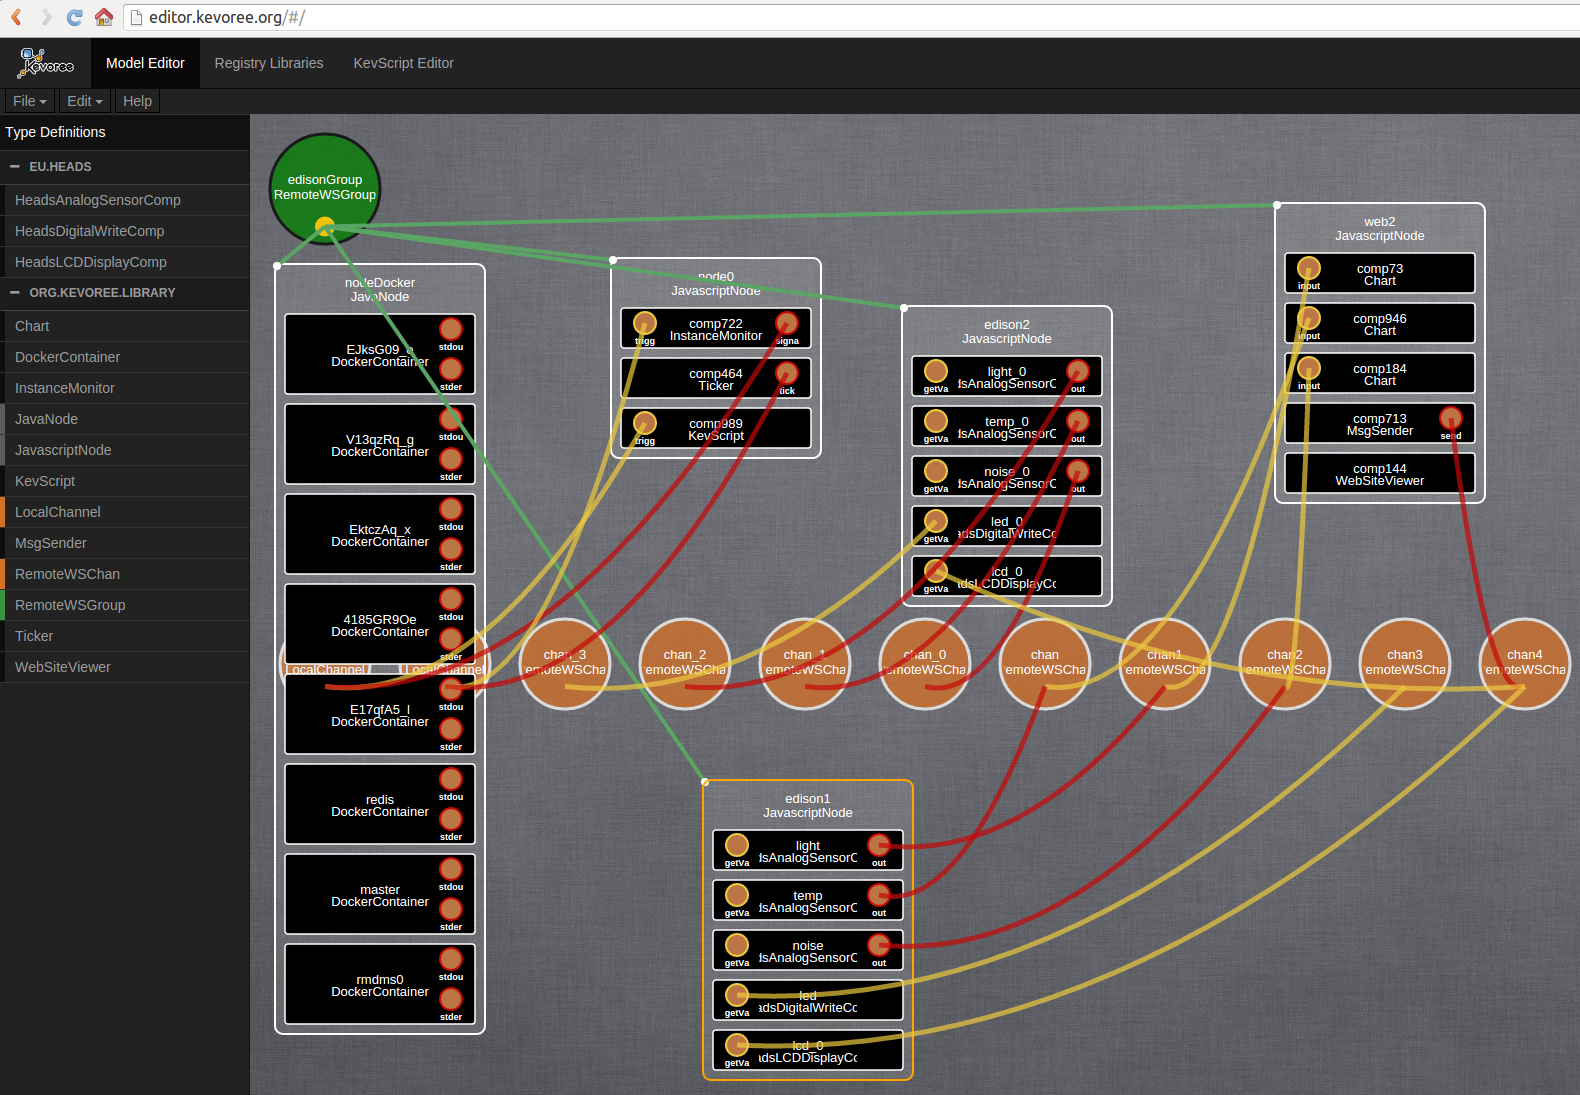
\includegraphics[width=1\linewidth]{figures/fig1}
	\caption{An example of dashboard for sensor-based applications}
	\label{fig:fig1}
\end{figure}


\begin{figure}[h]
	\centering
	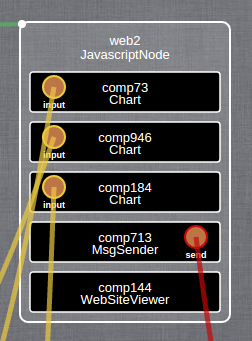
\includegraphics[width=0.5\linewidth]{figures/fig2}
	\caption{An example of sensor node based on Intel Edison}
	\label{fig:fig2}
\end{figure}


Starting the sensor based application on a Chrome browser, running on top of a HP EliteBook 820 with Intel i7 processor, SSD hard drive and 16Gbytes of memory, takes 1533 ms from scratch. It takes 677ms when the components are available in the cache. The load time is mainly the time to download software modules on the npm registry server. Deploying the sensor based dashboard consists in writing a simple configuration.    

\ff{Ideally here we could have a very nice graph. Like we could make vary the scale of the problem and measure the rendering/downloading/... time. This way we could conclude a bit more strongly about the overhead of browser rendering. Another point is that the server is also not under pressure to in theory we can serve more ... not easy to quickly monitor}

\subsubsection{Qualitative evaluation  }
To discuss the strength and the limitations of KevoreeJS, we can discuss the current approach regarding the challenges that have been discussed in Section 2.   

\indent \textbf{1.} KevoreeJS provides an initial solution to automatically provision component implementation and third-party libraries. It reuses Bower dependencies model to knows components dependencies and automatically download and install new components. It reuse npm registry to provide public access to the component implementation. KevoreeJS does not provide any sandboxing mechanisms for components. As a result, a KevoreeJS component can easily crash the full reconfigurable SPA. 

\indent \textbf{2.} KevoreeJS provides a basic type system inherited from the Kevoree component to check component assembly description. It also supports a development that can use TypeScript to ensure that a component is conforms to its interface.  

\indent \textbf{3.} KevoreeJS provides an initial UI composition mechanism based on mashup. If this UI composition mechanism is sufficient for a sensor based dashboard, KevoreeJS does not provides advanced composition mechanism.  

\indent \textbf{4.} KevoreeJS provides an initial solution to ensure that only some peers can change the configuration model. However, there is currently no solution to manage some role based access rules on the configuration models. Kevoree relies on registries, which are the providers of the model characteristics. It deal with the same issue of trustability the Linux distributions providers (e.g debian's apt, arch's linux pacman...) have encountered in the past (i.e. what happened if an attacker corrupt a registry and reference a malware?).  In its current implementation, by default, Kevoree is unsecured.   

\indent \textbf{5.} Search Engine Optimization is still an open problem. We do not provide new concepts in the KevoreeJS to solve this issue.    

\indent \textbf{6.} We support client/server partitioning. 11 among 14 modules that has been developed for the motivating scenario are cross-platform Java-JavaScript components, consequently they can run on the server side or on the client side.  One of the component for doing complex event processing is generated from ThingML behavioral description. ThingML~\cite{DBLP:conf/models/FleureyMSB11} provides code generators for Java, JavaScript, and C. Consequently this component can be deployed dynamically on the Browser or within a Java or JavaScript Kevoree runtime on the server.  

\indent \textbf{7.} We take the design decision in KevoreeJS that the browser history only affect the component states. We do not use Browser history API to go back to a previous SPA configuration. 

\indent \textbf{8.} We currently do not provide any solutions for improving analytics in dynamically adaptable SPA.   

\indent \textbf{9.} Finally, the core take 20kbytes without any minification. The use of KevoreeJS does not have any real impact on the SPA performance.



\section{Related Work}

Several component model exist for building dynamically adaptable web application. OSGi~\cite{hall2011osgi} provides an initial RFP for providing an OSGi for web applications. Eclipse provides an initial solution within the Orion project to write plugins for its online IDE~\footnote{http://wiki.eclipse.org/Orion}. However, this approach does not support dynamic reconfiguration without reloading the web pages.   ComponentJS~\footnote{http://componentjs.com/} is a stand-alone MPL-licensed Open Source library for JavaScript, providing a powerful run-time Component System for hierarchically structuring the User-Interface (UI) dialogs of complex SPA. It provides a rich component model for UI composition based on the concepts  of Event, Service, Hook, Model, Socket, and Property. However, it does not manage the dynamic reconfiguration of running applications. 
Lerner et al.~\cite{150010} present C3, an implementation of the HTML/CSS/JS platform designed for web-client research and experimentation. C3  explores the role of extensibility throughout the web platform for customization and research efforts. C3 proposes an interesting component model for the Web browser (the application container) itself. It proposes an extensible architecture to let developers to evolve the browser. 
Escoffier et al.~\cite{escoffier:hal-00854339} developed a service-oriented component framework, named H-ubu. Its purpose is to bring modularity to applications and to ease their runtime adaptation. H-ubu is based on the notion of components with provided and required services and on a hub, a specific component in charge with runtime components bindings. H-ubu  follows a dynamic service approach. Main adaptations consists in reacting when a component becomes unavailable but the framework does not provide specific mechanism to automatically deploy and remove required components. The configuration model is not explicit, as in a service oriented architecture, each hub manages dynamically the bindings between component services.
\section{Conclusion}
This paper highlights the motivations, challenges, and main requirements to build a dynamic component model for single page applications. It shows how a distributed system running on top of various browsers relying on heterogeneous hardware can be considered as a common service. This leads to the need of managing the configuration of such a service from a common and abstract view. This paper presents the requirements for such a system and KevoreeJS, an implementation of the Kevoree Component Model for the Browser. It evaluates KevoreeJS by building a dashboard for sensor-based applications that can be dynamically reconfigured. In particular, it supports dynamic client/server code partitioning and dynamic component installation without refreshing the web page.

We are currently extending this approach to improve security, to support analytic services and search engine optimizations. From a technical point of view, we are working on a pattern to support other SPA frameworks such as AngularJS 2 or React. In this direction, we are working on a development model that decreases the coupling between the  component implementation and the SPA application framework used to provide a clean MVC framework.  %We are also building a common taxonomy and a survey to compare all the component models that exist for SPA based on the criteria discussed in section 2.





% conference papers do not normally have an appendix


% use section* for acknowledgment
\section*{Acknowledgment}

The research leading to these results has received funding from the European Union Seventh Framework Programme (FP7/2007-2013) under grant agreement n611337, the HEADS project (www.heads-project.eu)




% trigger a \newpage just before the given reference
% number - used to balance the columns on the last page
% adjust value as needed - may need to be readjusted if
% the document is modified later
%\IEEEtriggeratref{8}
% The "triggered" command can be changed if desired:
%\IEEEtriggercmd{\enlargethispage{-5in}}

% references section

% can use a bibliography generated by BibTeX as a .bbl file
% BibTeX documentation can be easily obtained at:
% http://mirror.ctan.org/biblio/bibtex/contrib/doc/
% The IEEEtran BibTeX style support page is at:
% http://www.michaelshell.org/tex/ieeetran/bibtex/
\bibliographystyle{IEEEtran}
% argument is your BibTeX string definitions and bibliography database(s)
\bibliography{cbse}
%
% <OR> manually copy in the resultant .bbl file
% set second argument of \begin to the number of references
% (used to reserve space for the reference number labels box)





% that's all folks
\end{document}
